\chapter{Solution Overview}
\label{cha:implementation}


\section{A note on modularity}

The project as a whole was designed to be a application that allows for code analysis, however implementing abstractions from a level of reading bytes from process memory all the way to managing the interface's state resulted in the decision to split the deliverable into three separate entities named: reader, analyzer and bin (for binary). As the project was implemented in rust i was able to leverage rust's \verb|cargo| build system to easily manage all three projects as subdirectories

\begin{lstlisting}[caption="The basic project structure"]
/memspotter
    /reader
    /analyzer
    /bin
\end{lstlisting}

Furthermore to ease the usage and possible refactors i decided to use rust's \verb|trait| \footnote{\enquote{Traits are similar to a feature often called interfaces in other languages, although with some differences.} - The Rust Book} system to define shared function and type signatures which i could then implement for the data structures and abstractions of my choosing

\begin{lstlisting}[caption=\label{lst:arch}"a trait definition example", language=Rust,]
/// Defines an architecture for the program
#[blanket::blanket(derive(Ref, Rc, Arc, Box))]
pub trait Arch: Debug + Clone + PartialEq + Eq {
    /// the process id type usually a [u64]
    type Pid: Sized + Debug;
    /// the single instruction type
    type Instruction: Sized + Debug + From<u8>;
    /// the header type of the /maps file for the arch
    type Header: MapHeader;
}    
\end{lstlisting}

as seen in \ref{lst:arch} the Arch trait can even defines no new functions, but allow for defining that each architecture has an associated pid, instruction and header types. This in turn can be used to ease the later abstractions. 

\begin{lstlisting}[caption=\label{lst:segment}"The memory segment trait", language=Rust]
/// generic trait for a allocated memory segment of a process
pub trait MemorySegment<A>: Sized + std::fmt::Debug + Clone + Eq + PartialEq
where
    A: Arch,
{
    /// returns the segment's bytes
    fn memory(&self) -> &[u8];
    /// iterates over the segment's bytes
    fn iter_memory(&self) -> impl Iterator<Item = &u8>;
    /// returns the segment's header
    fn header(&self) -> &A::Header;
}
\end{lstlisting}

A great example of such ease would be the memory segment trait \ref{lst:segment} which can just take a given architecture implementation and it's specific header type will be included too, and can even be referenced in the function signatures (see the \verb|header(&self)| function).

Such design choice additionally allows for different implementations to expose a common interface but also be extremely flexible in the implementations as. for example the apple based \verb|Mach-O| objects can implement it only for their own specific architecture but the \verb|x86_64| family of systems can implement header for both the 64 and 32-bit ELF file variations. Furthermore it also allows for easy differentiation between globally shared behavior and architecture-specific implementation as can be seen in \ref{lst:reader_structure}.

\begin{lstlisting}[caption=\label{lst:reader_structure}"Structure of the reader module outlining separate trait and implementation folder"]
/reader
    ...
    /traits
        arch.rs
        map.rs
        header.rs
        function.rs
        library.rs
        ...
    /x864_64
        arch.rs
        map.rs
        header.rs
        so_function.rs
        shared_object.rs
        ...
        
\end{lstlisting}

\section{Reader module}
\label{reader}

\subsection{Traits}

\begin{figure}
    \centering
    
\includegraphics[width=0.65\linewidth]{reader_traits.drawio.png}
    \caption{Basic Diagram of Reader module trait dependencies and methods}
    \label{fig:reader-traits}
\end{figure}

the reader module at it's core beside the Arch \ref{lst:arch} and Segment \ref{lst:segment} traits is represented by a total of 6 traits which dependency can be observed in \ref{fig:reader-traits}.
\begin{enumerate}

    \item \label{reader:map}Map

Map is the most top level trait and fully abstracts over the contents of the entire process memory as well as the linked library code.
This trait allows access to the process pid, individual memory segments as described and read from the \verb|\proc\{pid}\maps| \cite{kerrisk_proc_pid_maps5_2024} specification.
It also allows the user to access the individual mapped libraries of the process \ref{reader:mapped_lib}.
It also defines special functions which return the special stack and heap segments \cite{TODO}.
    
\begin{lstlisting}[caption=\label{lst:map}"The Memory Map Trait definition", language=Rust]
 /// Describes a mapping of process part header to memory segments
#[blanket::blanket(derive(Ref, Rc, Arc, Box))]
pub trait Map<A: Arch + 'static>: Sized + Clone {
    /// map error type
    //type Error: std::error::Error;
    /// the specific memory segment type
    type Segment: MemorySegment<A>;
    /// the specific library type
    type Library: MappedLibrary<A>;

    /// returns the process pid
    fn pid(&self) -> A::Pid;

    /// returns segments
    fn segments(&self) -> Vec<Self::Segment>;
    /// returns an iterator ov the segments
    fn iter_segments(&self) -> impl Iterator<Item = Self::Segment>;

    /// returns the stack segment
    fn stack(&self) -> Self::Segment;
    /// returns the head segment
    fn heap(&self) -> Self::Segment;

    /// returns all segments that are linked
    //fn linked(&self) -> &[Self::Library];
    /// iterates over all segments that are linked
    fn iter_linked(&self) -> impl Iterator<Item = Self::Library>;
}   
\end{lstlisting}

 \item \label{reader:mapped_lib} MappedLibrary

    This trait is an abstraction that represents a system shared library that has been mapped onto segments of a running process.
    It defines methods that expose the actual library \ref{reader:library} as well as the ability to access the individual memory segments \ref{lst:segment}.
    For ease of use in analysis it also defines methods for directly accessing the writeable and executable segments directly, as well a a function which allows for translating the address of a library's function \ref{reader:function} to an address in the process memory space.
\begin{lstlisting}[caption=\label{lst:mapped_lib}"The MappedLibrary Trait definition", language=Rust]
 /// represents a memory segment that is linked from some library
#[blanket::blanket(derive(Ref, Rc, Arc, Box))]
pub trait MappedLibrary<A>
where
    A: Arch,
    Self: std::fmt::Debug + Clone,
{
    /// the library type that the segment is mapped to
    type Library: Library<A>;
    /// the memory segment type to which the library refers
    type Segment: MemorySegment<A>;
    /// returns the linked library reference
    fn library(&self) -> Self::Library;
    /// returns all of the segments
    fn segments(&self) -> Vec<Self::Segment>;
    /// iterates over the whole linked memory
    /// goes through segments in order, so breaks between addressed 
    /// will not be included
    fn iter_mem(&self) -> impl Iterator<Item = &u8>;

    /// retrieves the first found executable segment
    /// CAN PANIC
    fn exec_segment(&self) -> Self::Segment;
    /// retrieves the first found writable segment
    /// CAN PANIC
    fn write_segment(&self) -> Self::Segment;
    /// returns the mapped address of a function
    fn mapped_address(&self, func: &<Self::Library as Library<A>>::Function) -> u64;
}   
\end{lstlisting}
  
    \item \label{reader:library} Library
    
    This trait is a step lower on the abstraction ladder as it allows for the interaction with a shared library object.
    It exposes a definition of a specific implementation of the Function\ref{reader:function} trait that the library uses as well as methods that allow dumping the entire executable section memory as well as access to the range of the \verb|.text| section of the library file which holds the assembly code for the library's functions \cite{TODO}.
    Furthermore this trait allows for getting the function code from the library object for a function with a specific name as well as some helper methods such as \verb|fn name(&self) -> String| which returns the name of the shared library for ease of use.
    
\begin{lstlisting}[caption=\label{lst:library}"The Library Trait definition", language=Rust]
/// Trait for interacting with binary linkable objects e.g. `.so` files
#[blanket::blanket(derive(Ref, Rc, Arc, Box))]
pub trait Library<A: Arch>: Debug + Sized + PartialEq + Eq + Clone {
    /// the type for an individual library function
    type Function: Function<A>;
    /// type for the error the trait can return in functions
    type Error: std::error::Error;
    /// returns an [Iterator] over all instructions
    /// most likely in instruction order but not guaranteed
    fn instructions(&self) -> impl Iterator<Item = A::Instruction>;
    /// returns all [Self::Function]s contained in the library
    fn functions(&self) -> impl Iterator<Item = Self::Function>;
    /// returns a [Self::Function] for a given name if exists
    /// else returns [None]
    fn get(&self, name: &str) -> Option<&Self::Function>;
    /// returns the instruction [u8] and the [Self::Function] for a given index if inside library
    /// bounds
    fn context(&self, index: u64) -> Option<(&A::Instruction, &Self::Function)>;

    /// returns the file name of the library
    fn name(&self) -> String;

    ///returns the file address range for the `.text` section
    fn text_range(&self) -> std::ops::Range<u64>;
}
\end{lstlisting}  
    \item \label{reader:function} Function
    
    This trait defines the shared behavior of the Functions that a given library contains.
    It allows for both direct assembly code access to the whole function as well as specific ranges of it.
    Furthermore it exposes methods that allows for the name, size and more importantly location of the function in both a source file by providing the file offset as well as in a mapped process context by providing the virtual memory address.

\begin{lstlisting}[caption=\label{lst:function}"The Function Trait definition", language=Rust]
/// trait representing a function, usually from a [Library] context
#[blanket::blanket(derive(Ref, Rc, Arc, Box))]
pub trait Function<A: Arch>: Debug + Clone {
    /// returns the function name
    fn name(&self) -> String;
    /// returns the instruction range of the function e.g. its start and end
    fn file_context(&self) -> std::ops::Range<u64>;
    /// memory address at which the function starts
    fn address(&self) -> u64;
    /// returns an iterator over every byte 
    /// ([Self::Instruction]) of the function code
    fn bytes(&self) -> impl Iterator<Item = u8>;
    /// gets the instruction [u8] at a given Index
    /// returns [None] if index is out of bounds
    fn get(&self, index: u64) -> Option<&A::Instruction>;
    /// returns a given range of instructions ([\[u8\]])
    /// returns [None] if out of bounds
    fn range(&self, range: Range<u64>) -> Option<&[A::Instruction]>;
    /// returns the function size in bytes
    fn size(&self) -> u64;
    /// file offset
    fn file_offset(&self) -> u64;
}
\end{lstlisting}
    
    \item \label{reader:header}Header
    
    This trait defines the way of interaction with entries of the \verb|\proc\{pid}\maps| entries as defined in \cite{kerrisk_proc_pid_maps5_2024}.
    The included methods allow for accessing the mapped region's permissions, process memory range, the source file target as well as its offset and size. 
\begin{lstlisting}[caption=\label{lst:header}"The Header Trait definition", language=Rust]
/// Struct representing a single /mem/\<pid\>/maps entry
///
/// EXAMPLE
///
/// 35b1800000-35b1820000 r-xp 00000000 08:02 135522 /usr/lib64/ld-2.15.so
///
///  \[start\]-\[end\] \[permissions\] \[offset\] \[device\]:\[inode\] \[links_to\]
#[blanket::blanket(derive(Ref, Rc, Arc, Box))]
pub trait MapHeader: std::fmt::Debug + Eq + PartialEq + Clone + Ord {
    /// returns permissions
    fn permissions(&self) -> &Permissions;
    /// returns the mapped addresses described by the header
    fn mem_range(&self) -> std::ops::Range<u64>;
    /// returns the offset in the file or whatever it links to
    fn file_offset(&self) -> u64;
    /// size of the referenced memory in bytes
    fn mem_size(&self) -> u64;
    /// returns a string target for the header if exists
    fn target(&self) -> Option<String>;
}    
\end{lstlisting}
 
\end{enumerate}


\subsection{The header parsing process}

Firstly, the header is contained in one line and therefore can be derived from a string reference. This reference can then be split by space, however the space lengths can be varying and therefore the splitter needs to filter out the empty string fragments created by splitting multiple spaces joined together.
Next, values such as start, end or file offset are encoded in base 16 strings and therefore need to be parsed into integer types. 
Additionally the function employs a safety check to verify that the end is later than the start which ensures that the header string parsed is not malformed. 
Furthermore not all of the headers have a target section and therefore the last entry in splits section can be nonexistent.

\begin{lstlisting}
    fn try_from(value: &str) -> Result<Self, Self::Error> {
        let splits: Vec<&str> = value.split(' ').filter(|a| !a.is_empty()).collect();
        let [range, perms, offset, device, inode, ..] = splits[..] else {
            return Err(Self::Error::InsufficientInfo);
        };
        let [start, end, ..] = range.split('-').collect::<Vec<_>>()[..] else {
            return Err(Self::Error::InsufficientInfo);
        };
        info!("building header for range [{}-{}]", start, end);
        let start = u64::from_str_radix(start, 16)?;
        let end = u64::from_str_radix(end, 16)?;
        let offset = u64::from_str_radix(offset, 16)?;
        assert!(end >= start, "End cannot be earlier than start!");

        // read from the linked file
        let permissions = Permissions::try_from(perms)?;
        Ok(Self {
            start,
            end,
            permissions,
            offset,
            device: device.to_owned(),
            inode: inode.parse()?,
            target: splits.get(5).map(ToString::to_string),
        })
    }
\end{lstlisting}

\subsection{Memory Segments}

At the most base level the x86 Memory segment implementation is an enum which variants hold the respective segment structs. Most of those are just containers of bytes read from the memory.
However, the Linked segment variant holds a special implementation as this segment contains also an extra check to verify whether the target in the provided header is a valid file. 
The program uses the \verb|assert!| macro which will cause the program to panic when it is not fulfilled.
Furthermore separation segments into separate structs allows for defining special behavior, such as bypassing the memory reads and not inluding those structs in \verb|vvar| and \verb|vdso| segments as these are kernel space modules and cannot be read without privileged access (\cite{TODO}).

\subsection{Library implementation}

Firstly the specific layout of the library struct has been designed to minimize the memory impact of libraries.
Additionally the leveraging of smart pointer structures such as \verb|Box| or \verb|Rc| ensures that the actual contents of the memory live on the heap instead of the stack and reduce the memory footprint of the library struct.
Additionally the usage of reference counting pointers allows the consumers  of this struct to just clone the pointer and access the memory without memory heave copying operation or juggling pointers and their lifetimes to satisfy rust's memory protection constraints.

\begin{lstlisting}
/// representation for shared object parsed with the [goblin] crate
/// the addresses here are ABSOLUTE e.g. no offet introduced by linking
#[derive(Clone)]
pub struct SharedObject {
    functions: Box<[Rc<SoFunction>]>,
    memory: Rc<[u8]>,
    /// the `.so` name TODO
    path: PathBuf,
    text_offsets: Range<u64>,
}
\end{lstlisting}

As the library is usually inferred from a path included in the process memory segment header the library struct needs to parse this value to create itself which is done by implementing the \verb|try_from| method for the path buffer.
This method firstly leverages the file io access to read the file's contents to the provided buffer and then prasing the file's contents using the \verb|goblin| crate \cite{m4b_m4bgoblin_2024}.
This function call can also throw an error which will be propagated through the function call and let user know that the file is not a valid executable or a shared object.

\begin{lstlisting}
    fn try_from(value: PathBuf) -> Result<Self, Self::Error> {
        let mut file = std::fs::File::open(&value)?;
        let mut data = vec![];
        file.read_to_end(&mut data)?;
        let object = Object::parse(&data)?;
        let (text_offsets, text_vm_offsets) = Self::obj_text_ranges(&object)?;
        let functions: Vec<_> = Self::parse_object(&object, text_offsets.clone(), text_vm_offsets)?
            .into_iter()
            .map(|template| Rc::new(SoFunction::new(&data, template)))
            .collect();
        Ok(Self {
            path: value,
            memory: data.into_boxed_slice().into(),
            functions: functions.into_boxed_slice(),
            text_offsets,
        })
    }
\end{lstlisting}

Afterwards the the function calls the library's \verb|obj_text_ranges| \ref{} function which parses the provided object and extracting both text section offsets which allow to access sections of the file which contain the assembly functions that the library contains.
The function also provides more safety check as it returns an error when the provided object does not contain a .text section which makes the elf object invalid and unusable in the program context, as this section is responsible for containing the actual assembly code.
Additionally that function call also returns the range of the virtual memory to which the exported .text section maps in the process memory which will be immensely useful to match the code and function extracted from the library to code and functions extracted from the process memory.
This function also leverages that the object's produced by the gobl;in parser have enum variants representing different architecture and object types which opens up the possibility to provide architecture-specific parsing method while using a single function call.

\begin{lstlisting}
    /// returns the real and virtual memory adresses for the start of the `.text` elf file section
    //#[instrument]
    fn obj_text_ranges(
        object: &goblin::Object,
    ) -> Result<(Range<u64>, Range<u64>), crate::error::SharedObject> {
        match object {
            Object::Elf(elf) => {
                let text_section = elf
                    .section_headers
                    .iter()
                    .find(|section| {
                        elf.shdr_strtab.get_at(section.sh_name).unwrap_or("") == ".text"
                    })
                    .ok_or(crate::error::SharedObject::FileType(
                        "bad elf file - no .text section found".to_string(),
                    ))?;
                let text_start = text_section.sh_offset;
                Ok((
                    text_start..text_start + text_section.sh_size,
                    text_section.vm_range().start as u64..text_section.vm_range().end as u64,
                ))
            }
            ...
        }
    }
\end{lstlisting}

Lastly before returning the library object the function uses the \verb|parse_object| function to read from the object file all the functions that the library uses and then creates Function struct templates and later uses those templates to create actual function objects which are attached to the library struct as an array of pointers to these structs due to the usage of rc smart pointer.
In the x86 implementation his function makes heavy use of first the elf file's symbol table to get all the symbols that the library provides and filter it to provide only assembly functions which have a non-zero size.
Later the obtained symbols are translated into FunctionTemplate \ref{} objects with the usage of the provided text and virtual memory sectionns, and the size and symbol value obtained from the symbol table. 
The symbol value is later queried against elf's string table which allows to obtain the function name which concludes the creation of the function template.
After all of the templates are obtained they are collected into a vector struct and returned successfully from the function.

\begin{lstlisting}[language=Rust]
//#[instrument]
    fn parse_object(
        obj: &Object,
        text_range: Range<u64>,
        text_vm_range: Range<u64>,
    ) -> Result<Vec<FuncTemplate>, crate::error::SharedObject> {
        match obj {
            Object::Elf(obj) => {
            ...
                let d = span!(Level::INFO, "static_syms");
                let _guard = d.enter();
                let static_fns = obj
                    .syms
                    .iter()
                    .filter(|s| s.is_function() && !s.is_import())
                    .filter(Self::size_nonzero)
                    .filter(Self::nonalias)
                    .map(|sym| {
                        let mut start = sym.st_value;
                        if !obj.is_lib {
                            start = text_range.start + (sym.st_value - text_vm_range.start);
                        }
                        let name = obj
                            .strtab
                            .get_at(sym.st_name)
                            .unwrap_or("[UNKNOWN]")
                            .to_string();
                        let size = sym.st_size;

                        FuncTemplate {
                            memory_address: sym.st_value,
                            name,
                            file_offset: start,
                            size,
                        }
                    })
                    .collect();
                drop(_guard);
                Ok(static_fns)
            }
            ...
        }
    }    
\end{lstlisting}

\subsection{Function templates and Assembly functions}

Due to the Functio parsing process being split in two parts initially the Library parsing function only creates the function template instances \ref{} that contain only the function data that has been extracted from the function symbol as well as the function parent object's string and symbol table
\begin{lstlisting}
#[derive(Clone, Debug)]
pub struct FuncTemplate {
    pub name: String,
    pub memory_address: u64,
    pub file_offset: u64,
    pub size: u64,
}
\end{lstlisting}

The fully qualified function struct used in the library \ref{} code trades the offset and size fields for the start and end fields and additionally contains a box pointer to the function's bytes in the memory field of the struct.
\begin{lstlisting}
/// represents a singular function from the [SharedObject]
#[derive(Clone)]
pub struct SoFunction {
    name: String,
    start: u64,
    end: u64,
    mem_addr: u64,
    memory: Box<[u8]>,
}
\end{lstlisting}
The actual function struct creation process is started by providing the FuncTemplate and byte access to the library code. 
Afterwards the function creation method uses the data provided in the template to read the needed bytes from the library code and provide the function's context both within the file as well as the virtual address space by providing the start, end and memory address fields. 
\begin{lstlisting}
    impl SoFunction {
    /// creates a new insrance of the struct
    #[must_use]
    pub fn new(data: &Vec<u8>, template: FuncTemplate) -> Self {
        tracing::info!("creating function {:?}", template);
        assert_ne!(template.size, 0, "{} has 0 size", template.name);
        let end = template.file_offset + template.size;
        Self {
            name: template.name,
            start: template.file_offset,
            end,
            mem_addr: template.memory_address,
            memory: data[template.file_offset as usize..end as usize].into(),
        }
    }
}
\end{lstlisting}

\subsection{the library to memory mapping}

In order to facilitate verification of instructions in memory to instructions in shared objects the MappedLibrary struct has to be set up with care.
Firstly the struct needs to be extendable as a single library can be mapped to multiple process memory segments.
However this cannot be so straightforward and in this case if the segment supplied for extension does not place next in the process memory layout the program will panic in order to prevent inconsistencies in memory order and instruction analysis.
\begin{lstlisting}[caption=\label{mapped_lib:extend}"The extend function for the MappedLibrary struct", language=Rust, breaklines=true]
/// extends the linked memory with a provided segment
    pub fn extend(&mut self, segment: Linked<A>) -> &mut Self {
        match self.mapped_segments.last() {
            Some(s) => {
                assert!(s.header().mem_range().end <= segment.header().mem_range().start);
                self.mapped_segments.push(Rc::new(segment));
            }
            None => self.mapped_segments.push(Rc::new(segment)),
        }
        self
    }
\end{lstlisting}
Furthermore as the initializing function for this struct takes a valid existing Library \ref{lst:library} object it leaves this struct's only responsibility to align the library code with the segments.
\begin{lstlisting}[caption=\label{mapped_lib:new}"The creator function for the MappedLibrary struct", language=Rust, breaklines=true]
 /// initializes a new instance from a library object
    #[must_use]
    pub fn new(lib: L) -> Self {
        Self {
            library: Rc::new(lib),
            mapped_segments: Vec::new(),
        }
    }
\end{lstlisting}

Leveraging both the Segment \ref{} and Library \ref{} traits this struct can successfully bridge the virtual memory addresses from the shared object into real mapped addresses by the usage of mapped\_address function.
Furthermore this function is also adaptable to work on both shared objects and regular executables which do not leverage the virtual addresses and therefore file offset should not be applied.

\begin{lstlisting}[caption=\label{mapped_lib:mapped_addr}"The mapped\_address function for the MappedLibrary struct", language=Rust, breaklines=true]
fn mapped_address(&self, func: &<Self::Library as Library<A>>::Function) -> u64 {
        if self.library().name().contains(".so") {
            self.mapped_segments[0].header().mem_range().start + func.address()
        } else {
            func.address()
        }
    }
\end{lstlisting}



\subsection{x86\_64 Map implementation}

After the header parsing process the program opens the mem file.
Then for each of the header it first rewinds the memory file pointer to its starting position.
Then the method tries to create a memory segment \ref{lst:segment} specifically the x86 implementation of said interface \ref{lst:x86_segment} and propagates any encountered errors using the \verb|?| operator \cite{TODO}.
Afterwards the segment is wrapped into an Rc (reference counting pointer) which allows for easier access to the structure and more efficient memory usage. 
Then if the created segments ore of \verb|Linked| variant additional code tries to access the referenced file and create a MappedLibrary from it.
Additionally there the linked entries are extenden which mean that all segments of the linked object will be referencing a single library instance.
Lastly it is important to notice how rust's mutability rules are enforced - since the code creating the linked HashMap specifies the struct as mutable we cannot put them as-is into the ready map.
To match both the type and the non-mutability we have to iterate over the entries and wrap them in RC pointers too, they are static for the program lifetime and cannot be internally modified. 

\begin{lstlisting}[caption=\label{lst:map_from_pid}"Excerpt from x86\_64 Map's from\_pid function", language=Rust, breaklines=true]
/// creates a new instance from a provided process id
#[must_use]
#[instrument]
pub fn from_pid(pid: <X86_64 as crate::Arch>::Pid) -> Result<Self, crate::error::Error> {
    let mut linked = HashMap::new();
    let headers = ...
    ...
    let target = format!("/proc/{}/mem", pid);
    let mut mem_file = File::open(target).map_err(crate::error::Memory::from)?;
    let mut segments = Vec::with_capacity(headers.len());
    for header in headers {
        mem_file.rewind().map_err(crate::error::Memory::from)?;
        let reader = BufReader::new(&mem_file);
        let segment = X86_Segment::try_from((header, reader))?;
        segments.push(Rc::new(segment.clone()));
        if let X86_Segment::Linked(link) = segment {
        ...
            let lib = match Library::try_from(p.clone())
        ...
        linked
                    .entry(
                        link.header()
                            .target()
                            .expect("Linked segments shouuld ALWAYS have a valid target"),
                    )
                    .or_insert(MappedObject::new(lib))
                    .extend(link);
    }
    Ok(Self {
        pid,
        segments: segments.into_boxed_slice(),
        linked: linked.into_iter().map(|(k, v)| (k, Rc::new(v))).collect(),
    })
}
\end{lstlisting}

\section{Analyzer Module}
\label{analyzer}

\subsection{The analyzer trait}
\label{analyzer:trait}

The analyzer trait lies at the core of the analyzer crate and is responsible for providing a human readable output of the data read by the reader trait as well as providing some context to the read instructions. As it can be seen in the trait definition the only trait bounds \ref{}|\cite{} for the defined types are either \verb|Display| or \verb|Error| traits which allow basic interaction for any other programs.
Furthermore the trait defines the necessary methods for accessing the data with \verb|lib_instructions| and \verb|lib_context| methods which provide either the raw or context-annotated instruction access to specific libraries. 
Additionally the \verb|libraries| provide an easy access to the all included library \ref{} instances and a helper method to quickly access the main library of the process.

\begin{lstlisting}
    /// trait that defines the minimum functionality of different analyzers
pub trait Analyzer<M, A>
where
    A: Arch + 'static,
    M: Map<A>,
{
    /// the instruction type
    type Instruction: std::fmt::Display;
    /// the context that will accompany each instruction
    type Context: std::fmt::Display;
    /// the error type
    type Error: std::error::Error;
    /// returns the main usually the binary executable library
    fn main_lib(&self) -> M::Library;
    /// returns all libraries
    fn libraries(&self) -> Vec<M::Library>;
    /// returns the instruction of a given library (if such exists)
    fn lib_instructions(&self, lib: &M::Library) -> Result<Vec<Self::Instruction>, Self::Error>;
    /// returns the instructions accompanied iwth context of a given library
    fn lib_context(
        &self,
        lib: &M::Library,
    ) -> Result<Vec<(Self::Instruction, Self::Context)>, Self::Error>;
}
\end{lstlisting}

\subsection{diff\_analyzer implementation}

The analyzer trait implementation i settled on was aimed to provide context through differences between the code in the memory and the assembly code in the libraries.
At it's core i decided to use the capstone \cite{} disassembly framework as well as its rust bindings from the \verb|capstone-rs| crate \cite{finkenauer_capstone-rustcapstone-rs_nodate}.
The first stem in analyzer creation is to initialize the aforementioned dissasembler with the specified architecture for which it is implemented as well as setting the assembly syntax to intel and enabling detailed disassembly.
As the capstone disassembler initialization can also result in an error the cration function takes that into account and propagates it to the caller wrapped in its custom error type.
As the next step the function uses the provided process id to build the process memory map \ref{reader:map} and propagate any possible errors that may have occurred to to the caller.
Last step of note in the initialization process is the invocation of the \verb|create_func_map| function.

\begin{lstlisting}
    /// tries to initialize the analyzer from a provided process id
    #[must_use]
    pub fn from_pid(pid: usize) -> Result<Self, Error> {
        let disasm = Capstone::new()
            .x86()
            .mode(arch::x86::ArchMode::Mode64)
            .detail(true)
            .syntax(arch::x86::ArchSyntax::Intel)
            .build()
            .map_err(BuildError::from)?;
        let map = x86_64::Map::from_pid(pid as u64).map_err(BuildError::from)?;
        Ok(Self {
            pid,
            disasm,
            function_map: Self::create_func_map(&map),
            map,
        })
    }
\end{lstlisting}

This function is responsible for creating a HashMap structure which will allow the analyzer to easily access functions based on their process memory address.
To do this the method iterates over every function in every library, then extracts the function's mapped memory address using the \verb|mapped_address| \ref{mapped_lib:mapped_addr} function.
Furthermore to avoid address clashing only the latest read function is inserted to each address however this process is made transparent by emitting a warning to the logs notifying that a function is being replaced in the table.

\begin{lstlisting}
    fn create_func_map(memmap: &x86_64::Map) -> HashMap<u64, Rc<x86_64::Function>> {
        let mut map = HashMap::new();
        for l in memmap.iter_linked() {
            let span = warn_span!("func_map", lib = l.library().name());
            let _guard = span.enter();
            for f in l.library().functions() {
                let addr = l.mapped_address(&f);
                if let Some(rep) = map.insert(addr, f.clone()) {
                    tracing::warn!("clashing addresses replaced {:?} with {:?}", rep, f);
                }
            }
            drop(_guard);
        }
        map
    }
\end{lstlisting}

\subsection{The Instruction and Insight}

As seen in the analyzer trait \ref{analyzer:trait} the implementation needs a defined Instruction type. 
The type implemented for the diff analyzer implementation has contains only the three most important instruction information - the instruction address, mnemonic (such as \verb|mov|) and the instruction operands which are the arguments passed to the instruction.

\begin{lstlisting}
/// represents a single intel type instruction
#[derive(PartialEq, Eq, Clone)]
pub struct Instruction {
    /// the instruction address
    pub address: u64,
    /// the actual instruction or mnemonic
    pub instr: String,
    /// the instruction operands
    pub ops: String,
}
\end{lstlisting}

The creation of the Instruction instance from a capstone generated \verb|Insn| type is rather straight forward as the function just reads and calls unwrap on the instruction fields. 
To avoid the program panicking the unbwrap call substitutes a default string if the call would fail to avoid panic, however the calls are guaranteed to not fail per capstone-rs documentation as the avail;ability of them is gated by the \verb|detail| option of the dissasembler which is set to true in the \verb|diff_analyzer| initialization.

\begin{lstlisting}
impl<'a> From<&Insn<'a>> for Instruction {
    fn from(value: &Insn<'a>) -> Self {
        Self {
            address: value.address(),
            instr: value.mnemonic().unwrap_or_default().to_string(),
            ops: value.op_str().unwrap_or_default().to_string(),
            //regs_read: vec![],
            //regs_write: vec![],
        }
    }
}
\end{lstlisting}

TODO

\subsection{usage of the capstone crate and ffi}

As outlined in Section \ref{clean_code} the usage of \verb|unsafe| code inthe project is forbidden, however this does not propagate to the project's dependencies.
The most notorious breach of this rul;e occurs in the capstone-rs crate as it exposes binding for the capstone C library \cite{finkenauer_capstone-rustcapstone-rs_nodate}.
This however is rather necessary as there is no way of calling a foreign function interface (ffi) and guarantee rust's memory safety rules, hence the usage of unsafe code there is necessary.
Furthermore to ease the threat of memory leakage, the capstone-rs crate contains tests and the capstone framework itself is a well maintained open source library which actively deals with any program issues.

\subsection{extracting and matching the function addresses}

The core of the analyzer implementation functionality is comparing the memory code to the library code, and in order to do it the program has to know when to start matching which function in the memory instructions. 
In order to do that the program checks every address that it encounters against the previously created HashMap of function start addresses \ref{}.
If such an address is found the program loads the function from the library object and then disassembles it using the same disassembler it used for the memory code.
It also appends the function name to the context of the instruction to mark the function start.
Then the disassembled instructions are loaded into an iterator and kept outside the instruction loop.
Afterwards on every memory instruction encountered the program takes one instruction from the function instruction iterator and uses it for comparison as the addresses should match. 
Those two instructions are then used to generate the instruction Insight which provides information whether the instructions match addresses, mnemonics and operands.
This information is then appended to the context being created and returned along with the instruction.

\begin{lstlisting}
    lazy_static! {
    static ref FUNC_CALLS: [&'static str; 4] = ["jmp", "je", "jne", "call"];
}

\end{lstlisting}

\begin{lstlisting}
    fn lib_context(
        &self,
        lib: &Rc<x86_64::MappedObject>,
    ) -> Result<Vec<(Self::Instruction, Self::Context)>, Self::Error> {
        let mut data = vec![];
        let mut func = vec![].into_iter();
        for ins in self.lib_instructions(lib)?.into_iter() {
            let mut ctx = "".to_string();
            if let Some(f) = self.function_map.get(&ins.address) {
                ctx += &(f.name() + " ");
                let bytes: Vec<u8> = f.bytes().collect();
                let disasm = self
                    .disasm
                    .disasm_all(&bytes, ins.address)
                    .map_err(BuildError::from)?;
                func = disasm
                    .iter()
                    .map(Instruction::from)
                    .collect::<Vec<_>>()
                    .into_iter();
            }
            if FUNC_CALLS.contains(&ins.instr.as_str()) {
                if let Ok(addr) = u64::from_str_radix(&ins.ops[2..], 16) {
                    ctx += &format!(
                        "=>{} ",
                        self.function_map
                            .get(&addr)
                            .map(|f| f.name())
                            .unwrap_or(format!("{:#x} ", addr))
                    );
                }
            }
            if let Some(lib_asm) = func.next() {
                ctx += &Insight::from((&ins, &lib_asm)).to_string();
                ctx += " |"
            }

            data.push((ins, ctx.to_owned()))
        }
        Ok(data)
    }
\end{lstlisting}

\section{TUI program}

\subsection{the command line interface}

    - cli options

\begin{lstlisting}
    #[derive(Parser, Debug)]
#[command(version, about)]
struct Args {
    #[arg(required = true, value_name = "PROCESS_ID", index = 1)]
    pub process_id: usize,
    #[arg(
        required = false,
        value_name = "LOG_LEVEL",
        default_value = "warn",
        long = "log"
    )]
    pub log_level: Level,
}
\end{lstlisting}
    
    - autogenerated cli docs

    \begin{figure}
        \centering
        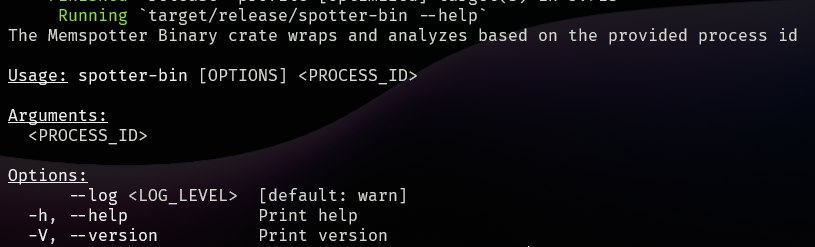
\includegraphics[width=0.5\linewidth]{cli-help.png}
        \caption{Running the binary with "--help" command}
        \label{fig:cli-help}
    \end{figure}

\subsection{the main interface}
- usage

- buffering the reader segments

- ui capabilities


\section{Enforcement of clean code principles}
\label{clean_code}

\begin{enumerate}
    \item Forbidding of \verb|unsafe| code
    
    Although rust is by definition a memory safe language due to the enforcement of the borrow checker and it's rules \cite{TODO}. However those features can be bypassed by the usage of \verb|unsafe| code blocks which disable these protection features at the programmers request.
    In the case of this project in order to enforce strict memory protection and avoid undefined behavior the \verb|unsafe_code| lint has been set to \verb|forbid| level which makes any usage of the unsafe blocks in the produced code emit a compile-time error which in no way can be overridden \cite{TODO - rust book}

    \item  Denying the use of \verb|unwrap()| calls

    One of the core features of the rust programming language is its verbosity in handling error cases, if a function can fail it usually returns a \verb|Result| which contains either the desired value or the error and needs to be handled appropriately \cite{TODO}. The same is applied for possible null values which hare handled with the \verb|Option| type which returns a \verb|None| variant to signify the lack of a result \cite{TODO}. 
    Those enforcements can be quickly bypassed by calling \verb|.unwrap()| on a \verb|Result| or an \verb|Option| value which will force the program to produce the desired value or fail and panic in the other case.
    To ensure better code quality and fewer panics in the implementation the \verb|unwrap_used| lint has been set at the \verb|deny| level. 
    This makes use of any \verb|unwrap| function calls result in a compilation error which forces the programmer to either handle the possible errors and None value accordingly or use the more verbose \verb|.expect()| call which requires an explanation to be provided to why the program should not panic when unwrapping this value \cite{TODO rust book}. 
    Furthermore by setting the \verb|expect_used| lint at a warning level the programmer will be still notified upon compilation that such method is not the best practice.

    \item Requirement of code documentation and other lints

    By setting the \verb|missing_docs| lint at a deny level the compiler will enforce that any public facing struct, enum, trait, and method needs to provide any documentation in order for the program to compile. This ensures that code not only need to be correct but also documented in order to be compiled and tested, which results in better documented and more maintainable code. 
    Furthermore by setting more specific lints such as \verb|clippy::pedantic| or \verb|clippy::nursery| the programmer is warned about bad code practices such as duplication module name in function or struct names or using less readable patterns such as \verb|if a != b|.
\end{enumerate}

\section{Custom error types}

Leveraging the use of the \verb|thiserror| crate \cite{tolnay_dtolnaythiserror_2024} the reader\ref{reader} and analyzer \ref{analyzer} modules expose custom error types which allow for better handling and displaying of any errors that occur. 
A good example of this is trying to read the memory of a process running with privileged access as a regular user (see \ref{lst:verbose_err}). Normally the resulted panic message would contain only the IO error produced by the access denied system response but with custom error type the message is more verbose.

\begin{lstlisting}[caption=\label{lst:verbose_err}"Error when trying to read the pid 1 process"]
Running `target/release/spotter-bin --log=error 1`
thread 'main' panicked at bin/src/main.rs:33:53:
Analyzer should init: Builder(
    Reader(
        MemFile(
            Parser(
                Os { code: 13, kind: PermissionDenied, message: "Permission denied" }
                ))))
\end{lstlisting}

Furthermore this allows any libraries that may depend on functions that emit such verbose errors to better respond to their occurrences and react accordingly. 
A good example of this is in the x86\_64 map trait \ref{reader:map} implementation in which the error thrown on failure of parsing a file which is not in a compatible format is caught and only emitted as a warning message instead of causing the entire program to panic.

\begin{lstlisting}[caption=\label{lst:err_handling}"Customm error handling example", language=Rust]
let lib = match Library::try_from(p.clone()) {
                Ok(lib) => lib,
                Err(e) => {
                    tracing::warn!(
                        "failure to parse file {} skipping function extraction ({})",
                        p.display(),
                        e
                    );
                    continue;
                }
            };
\end{lstlisting}

Additionally by usage of custom error types the test suite of the program can be enhanced with purposefully panicking code which passes the test only on specific error types.

\section{Tracing}

By incorporating the \verb|tracing| \cite{tokio-rs_team_tokio-rstracing_2024} dependency into the reader \ref{reader} and analyzer \ref{analyzer} modules the exposed methods can produce tracing information which can be used and consumed by other libraries

\begin{lstlisting}[language=Rust, caption="Code fragment showcasing conditionally emiting a warning"]
if let Some(rep) = map.insert(addr, f.clone()) {
    tracing::warn!("clashing addresses replaced {:?} with {:?}", rep, f);
}
\end{lstlisting}

The binary module uses the \verb|tracing_subscriber| \cite{tokio-rs_team_tokiotracingtracing-subscriber_2024} crate to consume the data provided by it's function as well as it's dependencies and with the CLI setup to allow for trace level filtering the program can emit desired information to the end user.

\begin{lstlisting}[breaklines=true, caption="Fraction of the warnings emitted by the program with the log setting at warning level"]
$ cargo run --release -- --log=warn 5293
...
2025-01-05T15:27:26.763134Z  WARN func_map{lib="ld-linux-x86-64.so.2"}: memspotter_analyzer::diff_analyzer: clashing addresses replaced sbrk 0x22d10[139] with __sbrk 0x22d10[139]
2025-01-05T15:27:26.763153Z  WARN func_map{lib="ld-linux-x86-64.so.2"}: memspotter_analyzer::diff_analyzer: clashing addresses replaced __GI_mprotect 0x24800[36] with mprotect 0x24800[36]
2025-01-05T15:27:26.763172Z  WARN func_map{lib="ld-linux-x86-64.so.2"}: memspotter_analyzer::diff_analyzer: clashing addresses replaced access 0x241c0[55] with __access 0x241c0[55]
2025-01-05T15:27:26.763191Z  WARN func_map{lib="ld-linux-x86-64.so.2"}: memspotter_analyzer::diff_analyzer: clashing addresses replaced __closedir 0x22e80[44] with closedir 0x22e80[44]
2025-01-05T15:27:26.763211Z  WARN func_map{lib="ld-linux-x86-64.so.2"}: memspotter_analyzer::diff_analyzer: clashing addresses replaced __GI___fstatat 0x24240[76] with __GI___fstatat64 0x24240[76]
\end{lstlisting}